\chapter{Theory}
\label{chapter:theory}
\epigraph{\textit{Wir wollen immer da hin, wo jeglicher Druck mal ein Ende hat
Ha'm immer tausend Sachen auf'm Zettel, sach' ma', kennst du das?}}{Deichkind}

The starting point to study fluid dynamics is the Navier-Stokes equation~\cite{Navier, Stokes}, as motivated in Chap.~\ref{chapter:intro}.
Both Claude Navier in 1823 as well as Gorge G. Stokes in 1842 derived the momentum equation for a Newtonian liquid.
Historically these two were not the only ones. 
Siméon Denis Poisson and Barré de Saint-Venant came to the same conclusion around the same time~\cite{https://doi.org/10.1002/andp.18321010607, de1843notea, anderson_jr_1997}.
But history is crude and Navier as well as Stokes are identified with the derivation of the momentum of a fluid element. 

\section{Navier-Stokes}
\label{sec:navier_stokes_sec}
Mathematically the Navier-Stokes equation can be derived from one definition and two constraints.
The two constraints are mass and momentum conservation.
Mass conservation simply states that mass can not be destroyed or created.
The same argument holds for the momentum.
By Nöthers theorem every conserved quantity yields a symmetry and vice versa.
In this case conservation of momentum allows us to use the constraints on the solutions that translational symmetry requires.
Independent of my position in the office, either being at spot \textit{A} or \textit{B} the experiment, according to protocol, should yield the same result.
The last ingredient for the derivation is the definition of a fluid.
In fact this is a really hard one. 
To shorten the discussion a fluid is ``\textit{a substance that flows and is not solid}`` according to the Cambridge Dictionary.
This definition can be refined, because a fluid is either a gas or a liquid that continuously deforms under shear stress, at least a Newtonian fluid.
Meaning one finds a linear relation between shear rate and shear velocity.
Clearly there are other liquids (which encloses granular systems to some extent) that exhibit different behaviour, for example think about toothpaste.
As long as there is no force applied to the tube the toothpaste does not flow.
Even the acceleration due gravity when pointing the tube towards the ground does not exert enough force to generate a flow.
In contrast to Newtonian liquids those liquids have a different response function to shear, they can be addressed as \textit{power law} fluids.
While the phenomenology of these fluids, e.g. shear thinning or thickening, is very interesting it is beyond the scope of this work. 
That said in Chap.~\ref{chapter:second_paper} an extension towards more complex flows is presented. 
In this specific case the addition of thermal noise to approximate the stochastic thin film equation (STF).
Chap.~\ref{chapter:second_paper} should serve as a guideline for further features, such as viscoelasticity for non-Newtonian liquids~\cite{doi:10.1142/S0218202513500140}. 

Knowing what a fluid is and taking into account the conservation of mass and momentum it is possible to derive the Navier-Stokes equation. 
Starting with the continuity equation that states that the fluid itself is a continuum and ignoring the underlying molecular structure for now. 
Meaning that the fluid can be described with a density $\rho(\mathbf{x},t)$.
Assuming an infinitesimal small volume of fluid $V_0$ its density can only change if there is a flow through the boundaries of the volume $\partial V_0$,
\begin{equation}\label{eq:cont_1}
    \partial_t\int_{V_0}\rho\diff V = -\oint_{\partial V_0} \rho\mathbf{u}\cdot\diff \textbf{A}, 
\end{equation}
where $\mathbf{u}(\mathbf{x},t)$ is the fluids velocity, A is the area that encloses the volume $V_0$ and $\diff\textbf{A}$ are the normals pointing outwards of the volume.
Violations of this Eq.~(\ref{eq:cont_1}) are equivalent to generation or destruction of mass.

Thanks to Gauss the integral over a closed surface can be written as divergence of a volume and thus the above equation becomes
\begin{equation}\label{eq:cont_2}
    \partial_t\int_{V_0}\rho\diff V = -\int_{V_0} \nabla\cdot(\rho\mathbf{u}) \diff V. 
\end{equation}
Since both sides are integrals over the volume $V_0$ we drop them and work with the differential equation
\begin{equation}\label{eq:cont_3}
    \partial_t\rho + \nabla\cdot(\rho\mathbf{u}) = 0,
\end{equation}
which will be addressed as the continuity equation through the thesis.
Actually one finds this equation not only in fluid dynamics for mass conservation but as well in electrodynamics for charge conservation, where the second term is often refereed to as flux~\cite{jackson1999classical, griffiths2005introduction}.

For the momentum equation the same line of argument is applied, however momentum can change for different reasons.
First being that momentum is advected from or into the volume $V_0$.
Pressure on the other hand can be a source of momentum and of course forces that are applied to the fluid are as well sources~\cite{krueger2017}.
Collecting these terms and writing down an equation for the momentum one gets,
\begin{equation}\label{eq:navier_stokes_1}
    \partial_t \int_{V_0}\rho\mathbf{u}\diff V = -\oint_{\partial V_0}(\rho\mathbf{u}\mathbf{u})\cdot\diff\textbf{A} - \oint_{\partial V_0} p\diff\textbf{A} + \int_{V_0} \textbf{F}\diff V, 
\end{equation}
where $\mathbf{u}\mathbf{u}$ is used to denote the outer product.
Using the divergence theorem again to reformulate everything in terms of volume integrals and dropping the integration the above equation becomes
\begin{equation}\label{eq:navier_stokes_2}
    \partial_t(\rho\mathbf{u}) = -\nabla\cdot(\rho\mathbf{u}\mathbf{u}) - \nabla p + \textbf{F}.
\end{equation}
This however is not yet the Navier-Stokes equation, in fact this is the Euler equation~\cite{batchelor2000introduction}.
In the derivation there is one term missing, because the momentum of a fluid can also change due to internal friction, or put simply, due to viscosity.
This viscous contributions are collected in the viscous stress tensor $\hat{\sigma}$ as
\begin{equation}\label{eq:stress_tens}
    \hat{\sigma}_{ij} = \mu\left(\frac{\partial u_i}{\partial x_j} + \frac{\partial u_j}{\partial x_i}\right) + \lambda\delta_{ij}\frac{\partial u_k}{\partial x_k},
\end{equation}
Actually this tensor introduces a lot of the complexity of the Navier-Stokes equation as in principle neither $\mu$ nor $\lambda$ need to be constants and in fact they are tensors themselves.

For the sake of clarity however here it is assumed that both $\mu$ and $\lambda$ are constants.
Inclusion of pressure to $\hat{\sigma}$ yields the total stress tensor $\tilde{\sigma}$. 
Due to symmetries of the problem there are various constraints on this tensor.
A fluid element can be stretched and rotated, because it is allowed to deform in contrast to a solid body.
However working out these constraints the pressure has to be a diagonal term and thus
\begin{equation}\label{eq:total_stress}
    \tilde{\sigma}_{ij} = - p \delta_{ij} + \mu\left(\frac{\partial u_i}{\partial x_j} + \frac{\partial u_j}{\partial x_i}\right) + \lambda\delta_{ij}\frac{\partial u_k}{\partial x_k}.
\end{equation}
Adding the viscous part of the tensor to the momentum equation Eq.~(\ref{eq:navier_stokes_2}) and rearranging terms,
\begin{equation}\label{eq:navier_stokes_3}
    \partial_t(\rho\mathbf{u}) + \nabla\cdot(\rho\mathbf{u}\mathbf{u}) = - \nabla p + \nabla\left[\mu(\nabla\mathbf{u} + \nabla\mathbf{u}^T) + \left(\eta-\frac{2\mu}{3}\right)\nabla\cdot\mathbf{u}\right] + \textbf{F},
\end{equation}
where we have used the differential form of Eq.~(\ref{eq:total_stress}) and $\lambda = \eta - 2/3\mu$.

Instead of trying to solve this, some words of reasoning.
The main goal of this thesis is to model the dynamics of thin film flows.
An area of fluid dynamics usually addressed as creeping flows. 
The flow velocities in this regime are in fact much slower than the speed of sound $c_s$ ($c_s^{\ce{H2O}} = 1500m/s $). 
This allows for the simplification of an incompressible medium.
For such media or fluids one can assume that $\rho = const.$ and therefore by Eq.~(\ref{eq:cont_3}) 
\begin{equation}\label{eq:incomp}
    \nabla\cdot\mathbf{u} = 0.
\end{equation}
A note of caution, while a constant density ($\rho = const.$) does satisfy the incompressibility constraint it is not unique to the underlying thermodynamics.
The thermodynamic compressibility $\kappa$ measures the change of volume with pressure and is given by 
\begin{equation}
    \kappa = \left(\frac{\partial V}{\partial p}\right)_T.
\end{equation}
Strictly speaking a fluid is incompressible as long its density does not depend on the pressure $p$ or $\kappa = 0$.

Inserting this constraint Eq.~(\ref{eq:incomp}) into Eq.~(\ref{eq:navier_stokes_3}) yields therefore the Navier-Stokes equation for an incompressible fluid as
\begin{equation}\label{eq:navier_stokes_4}
    \rho(\partial_t\mathbf{u} + \nabla\cdot\mathbf{u}\mathbf{u}) = - \nabla p + \mu\Delta\mathbf{u} + \textbf{F}.
\end{equation}
The left hand side can be rewritten using the material derivative
\begin{equation}\label{eq:mat_dev}
    D_t = \partial_t + \mathbf{u}\cdot\nabla, 
\end{equation}
which is a convenient measure for following a fluid element instead of a single point.
Inserting this, Eq.~(\ref{eq:navier_stokes_4}) can be written as
\begin{equation}\label{eq:navier_stokes_fin}
    \rho D_t \mathbf{u} =  - \nabla p + \mu\Delta\mathbf{u} + \textbf{F},
\end{equation}
where the symbol $\Delta$ denotes the Laplace operator.
Eqs.~(\ref{eq:cont_3}, \ref{eq:navier_stokes_4}) can not be solved because there are too few equations for too many unknowns.
So far there are five unknowns ($\rho, \mathbf{u}, p$) for four equations.
The clever way out of this misery is to use an equation of state that relates pressure, density, temperature, energy and entropy.
Especially the relation between pressure, density and temperature helps in closing the system of equations.
To define an equation of state is far from trivial.
It requires a thermodynamically consistent approach that is based on observations or theoretical assumptions.
The equation of state for an ideal gas was born from theoretical assumptions, e.g. non-interacting gas molecules, and reads~\cite{schwabl2006statistical}
\begin{equation}\label{eq:eq_of_state}
    p = \rho R T,
\end{equation}
where $R$ is the specific gas constant and $T$ is the temperature.
Having a well defined state in the thermodynamics sense allows to relate pressure and density and therefore to close the system of equations.
The equation of state for an ideal gas, see Eq.~(\ref{eq:eq_of_state}), will be revisited in Chap.~\ref{chapter:method} where we discuss the lattice Boltzmann method.

The Navier-Stokes equation, see Eqs.~(\ref{eq:cont_3}, \ref{eq:navier_stokes_4}), offers a general framework to deal with fluid dynamics problems.
As stated in the Chap.~\ref{chapter:intro} a general solution to this equation in a strictly mathematical sense is still missing and in fact worth a million dollars (and probably even more in an industrial setting).
For the concrete example of thin film flows however there is no need to ``solve'' the Navier-Stokes equation.
That is why in the next two sections different theories that build upon the Navier-Stokes are introduced.
Both of these theories using a scaling argument to severely simplify the resulting system of equations.

\section{Shallow Water Theory}
\label{sec:theory_shallow_water}
Solving the Navier-Stokes equation for the problems discussed in Chaps.~\ref{chapter:fourth_paper}-\ref{chapter:third_paper} is not needed.
Looking at Figs.~\ref{fig:examples_intro}-\ref{fig:morph_transition} one can identify that the height or thickness of the fluid layer is much smaller than the horizontal extension of the substrate.
This statement with some more approximations allow to derive another system of equations from the Navier-Stokes equation, the shallow water or Saint-Venant equations~\cite{saint1871theorie}.

\subsection{Definition}
\begin{figure}
    \centering
    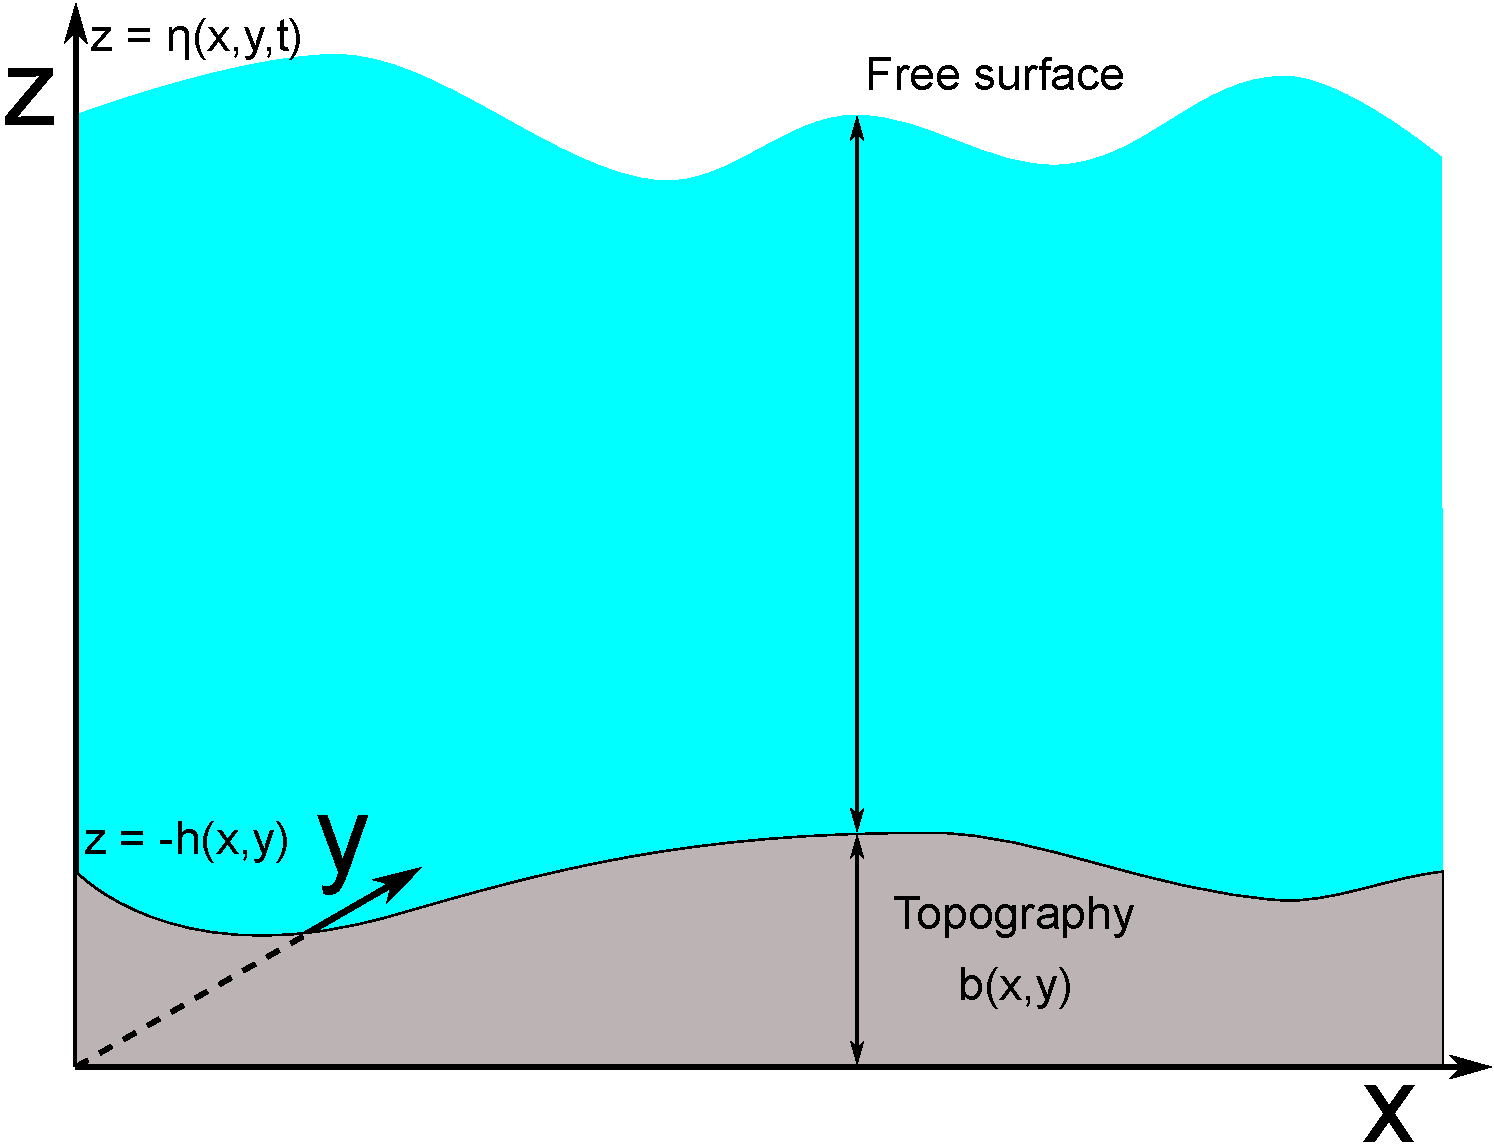
\includegraphics[width=0.95\textwidth]{graphics/simple_shallow_water.pdf}
    \caption{Schematic description of the shallow water problem. A liquid column with position of the free surface $\eta(x,y,t)$ covers a bottom topography $b(x,y)$.
    The liquid's height with the addition of the elevation of the topography defines the resulting height or z-component.}
    \label{fig:shallow_water_drawing}
\end{figure}

The shallow water model is a well working approximation to describe \textit{shallow} flows~\cite{tan1992shallow} and illustrated in Fig.~\ref{fig:shallow_water_drawing}.
Shallow by definition of the Cambridge dictionary means ``\textit{having only a short distance from the top to the bottom}``, which in fact describes quite well what the model does.
Instead of having a fully resolved three dimensional model of the fluids density and velocity the shallow water approach assumes that the degrees of freedom in the vertical direction can be integrated out. 
Therefore all dynamics of the system are effectively captured by the evolution based on the horizontal degrees of freedom $(x,y)$.

To make such strong assumptions it is necessary to take a look at the system at hand.
Coming back to the meaning of the word shallow, a shallow flow with a liquid column of height $h$ and horizontal length scale $L$ need to satisfy
\begin{equation}\label{eq:thickness_length}
    \varepsilon := \frac{h}{L} \ll 1,
\end{equation}
where $\varepsilon$ is a measure for the difference between those two scales.
An illustrative example that satisfies this inequality is any of the three major oceans.
On average they are $3000m$ deep but cover about $71\%$ of the earth's surface area which is approximately $361000000km^2$.
Dividing this number by three, to separate between Atlantic, Pacific and Indian ocean one gets a square with a side length of $~11000km$.
Inserting numbers in Eq.~(\ref{eq:thickness_length}) yields a ratio $\varepsilon \approx 3\cdot 10^{-4}$.
Meaning that the average height of the fluid column is negligibly small as compared to its horizontal scales.
Therefore the dynamics in vertical direction can be considered instantaneous. 
Interestingly the atmospheric layer satisfies this constraint as well. 
Some of its dynamics can be described with the shallow water model, at least to some extent.

Secondly comes the assumption of the pressure free surface.
Putting it simply, the shallow water model does not know what happens above the fluid.
The assumption is that the density of the layer above the fluid column is small compared to the fluid density.
Taking again the picture of the ocean, the density of (salt) water is around a thousand times higher than the density of the air above ($\rho^{\ce{H2O}} \approx 1000$kg/m$^3$, $\rho^{\text{air}} \approx 1,25$kg/m$^3$).
To some extent this is, again, actually true for the atmospheric layer.
Using the barometric formula to relate the density with altitude,
\begin{equation}\label{eq:bareometric_form}
    \rho(h_1) = \rho(h_0)e^{-\frac{\Delta h}{h_s}},
\end{equation}
with $\Delta h = h_1 - h_0$ and $h_s = RT/Mg$ is the scale height.
Of course, the model can be refined with a so called multi layer approach~\cite{tubbs2009multilayer, prestininzi2013effect}, but by definition the assumption is that upper end of the fluid column does not feel any pressure from above~\cite{tan1992shallow, james2019towards}.

Third, the horizontal velocity of the fluid has to vanish at the ``solid'' ground, or in terms of Fig.~\ref{fig:shallow_water_drawing} looking down from the free surface at $-h(x,y)$.
Meaning that although there is a viscosity associated with the fluid, friction with the bottom topography is the dominating dissipation channel.
Usually this kind of boundary condition is called \textbf{no-slip} boundary condition~\cite{richardson_1973, doi:10.1021/la0116342, Salmon:1999:0022-2402:503}.
While this may seem counterintuitive because fluid has no problem to flow over yet dry surfaces, modelling wetting or the wet-dry transition is a complex task, as seen later in this chapter and in Chaps.~\ref{chapter:first_paper}.
After all, a theoretical model which is defined as a set of partial differential equations can not account for the true complexity of nature~\cite{scriven_1988}.
We come back to the idea of the no-slip boundary condition in Sec.~\ref{sec:thin_films}.

And forth and observation concerning the vertical velocity.
Taking the oceans one more time as an illustrative example.
The big circular flow systems in the oceans like the gulf stream have much larger velocity components in the horizontal directions as compared to the vertical one.  
This is actually crucial to know because in the following mathematical modelling it is taken into account and will allow for further reduction of complexity.

How to make the Navier-Stokes equation, Eq.~(\ref{eq:navier_stokes_4}), aware about these constraints?
Partial differential equations are complex. 
They are one of the topics in mathematics where researchers are satisfied with the irritating result that an equation can not be solved, an undesired outcome for most Physicists.
Nevertheless, to come up with consistent strategies to solve them one can classify them, e.g. hyperbolic, parabolic, linear, nonlinear, initial value problem or boundary value problem.
There is in fact overlap between those terms, however to keep things simple it is sufficient to talk about initial or boundary value problems.
The former can be solved knowing the initial configuration which then defines the evolution, e.g. the initial coordinates and velocity of a pendulum. 
For the later ones it is mandatory to know the solution at the boundaries, e.g. the heat distribution in a solid body where it is needed to know the temperatures at the boundaries of the solid.
The Shallow water system can be derived from the Navier-Stokes using both well defined boundary conditions and system specific approximations.
For example the statement \textit{pressure free surface} means that there is a boundary condition that requires $p = 0$ at $z = \eta$, therefore there is no pressure acting on liquids interface.

\subsection{Scaling analysis}
\label{subssec:scaling_shallow water}
Starting with the system specific approximations, in Eq.~(\ref{eq:thickness_length}) a so-called scaling parameter $\varepsilon$ has been introduced. 
Using this parameter to rescale the velocities, because we know that the horizontal velocities are large as compared to the vertical
\begin{equation}\label{eq:vel_scaling}
    u_x = \tilde{u}_x,\quad u_y = \tilde{u}_y,\quad u_z = \varepsilon\tilde{u}_z.
\end{equation}
For an incompressible fluid with vanishing density gradient Eq.~(\ref{eq:cont_3}) therefore becomes
\begin{equation}\label{eq:cont_nondim}
    \nabla\cdot\mathbf{u} = \partial_x u_x + \partial_y u_y + \varepsilon\partial_z u_z = 0.
\end{equation}
To satisfy that all terms of this equation are the same order in $\varepsilon$ the coordinates need to be rescaled as well. 
This choice however is not unique and offers two possibilities~\cite{james2019towards}.
There is on the one hand the long wave approximation~\cite{RevModPhys.69.931},
\begin{equation}\label{eq:long_wave_scaling}
    x = \frac{\tilde{x}}{\varepsilon},\quad y = \frac{\tilde{y}}{\varepsilon},\quad z = \tilde{z},\quad t = \frac{\tilde{t}}{\varepsilon},
\end{equation}
which again is encountered in Sec.~\ref{subsec:thin_film_scaling} and tries to smooth out spatial and temporal variations.
On the other hand is the thin layer scaling
\begin{equation}\label{eq:scaling_thin_layer}
    x = \tilde{x},\quad y = \tilde{y},\quad z = \varepsilon\tilde{z},\quad t = \tilde{t},
\end{equation}
which correspond to the classical scaling of boundary layer theory~\cite{milne1996theoretical}.

In Eqs.~(\ref{eq:vel_scaling}-\ref{eq:scaling_thin_layer}) there is no distinct difference between both horizontal dimensions $(x,y)$. 
For the sake of clarity and to simplify the derivation of the shallow water model we neglect the $y$-components.
Of course, to study large oceanic systems or Coriolis forces one needs both horizontal dimensions, see e.g.~\cite{doi:10.1063/1.2116747, MARCHE200749}, but for the following derivation it is sufficient to use one.
Further we use the long wave approximation (or scaling, or theory), Eq.~(\ref{eq:long_wave_scaling}), we encounter it again in the thin film derivation.
The benefit of this choice is the smoothing effect on variations which makes them more gradual. 
On the same aspect the time also picks up a $1/\varepsilon$ contribution to smear out the dynamics.
Inserting Eqs.~(\ref{eq:vel_scaling},\ref{eq:long_wave_scaling}) into Eq.~(\ref{eq:cont_3}) yields
\begin{equation}\label{eq:rescaled_cont}
    \tilde{\vec{\nabla}}\cdot\tilde{\vec{u}} = \partial_{\tilde{x}} \tilde{u}_x + \partial_{\tilde{z}} \tilde{u}_z  = 0,
\end{equation}
where two dimensional vectors, such as $\vec{u} = (u_x, u_z)$ are denoted with an arrow symbol on top.

Scaling analysis and renormalization are key concepts in modern physics~\cite{yakhot1986renormalization, peskin2018introduction}.
One of the key concepts of this idea are symmetries, and therefore transformations under which a given state does not change.
Fluid dynamics to some extent admits a conformal symmetry.
The governing equations describe the flow through a nanotube as well as the circular currents in oceans~\cite{Secchi2016, MARCHE200749}.
Some features however such as the drag on an airfoil do not simply scale with the size of the system.
Therefore while a miniaturised model may create enough lift force, simply scaling up the size is not sufficient to ensure enough lift.  
In the following it will be helpful to introduce dimensionless numbers~\cite{ruzicka2008dimensionless,de1991fluid}.
These numbers have a long history in fluid dynamics, because only with them is it possible to compare experiments.
The ones of interest for the shallow water theory are the Reynolds number and the Froud number
\begin{equation}\label{eq:Re_and_Fr}
    Re = \frac{\rho L v_0}{\mu},\quad Fr = \frac{v_0}{\sqrt{g L}},
\end{equation}
where $L$ is a characteristic length scale of the problem, e.g. the mean water depth of a lake at rest, $v_0$ and $g$ are a characteristic velocity and the gravitational acceleration ($g = 9.81 m/s^2$) respectively.
A characteristic velocity can be for example the inflow velocity to a lake, or the speed of a certain wave type such as a tsunami.
Both numbers measure the magnitude of certain effects, in the case of the Reynolds number the inertia forces are compared against viscosity.
The Froud number is a measure to compare kinetic ($v_0$) with potential energy ($g L$).

In the next step both Fr and Re are used to make Eq.~(\ref{eq:navier_stokes_fin}) dimensionless.
For convenience the vector equation is split into two respective equations with gravity being the only force present.
Writing the full equation with all components yields
\begin{align}\label{eq:2d_RNS}
    \partial_t u_x + u_x\partial_x u_x + u_z\partial_z u_x &= -\partial_x p + \frac{1}{Re}\Delta u_x ,\\
    \partial_t u_z + u_z\partial_x u_x + u_z\partial_z u_z &= -\partial_z p - \frac{1}{Fr^2} + \frac{1}{Re}\Delta u_z ,
\end{align}
with the two dimensional Laplacian $\Delta = (\partial_x^2 + \partial_z^2)$.
Using long wave scaling, Eq.~(\ref{eq:long_wave_scaling}) and the rescaled length and time variables (e.g. $\tilde{x}$),
\begin{align}\label{eq:2d_RNS_eps}
    \varepsilon(\partial_{\tilde{t}} \tilde{u}_x + \tilde{u}_x \partial_{\tilde{x}} \tilde{u}_x + \tilde{u}_z \partial_{\tilde{z}} \tilde{u}_x ) &= -\varepsilon\partial_{\tilde{x}} \tilde{p} + \frac{1}{Re}(\varepsilon^2 \partial_{\tilde{x}}^2 \tilde{u}_x + \partial_{\tilde{z}}^2 \tilde{u}_x ) ,\\
    \varepsilon^2(\partial_{\tilde{t}} \tilde{u}_z + \tilde{u}_z\partial_{\tilde{x}} \tilde{u}_x + \tilde{u}_z\partial_{\tilde{z}} \tilde{u}_z) &= -\partial_{\tilde{z}}\tilde{p} - \frac{1}{Fr^2} + \frac{\varepsilon}{Re}(\varepsilon^2 \partial_{\tilde{x}}^2 \tilde{u}_z + \partial_{\tilde{z}}^2 \tilde{u}_z ) .
\end{align}
The scaling parameter $\varepsilon$ is a measure for the relation between thickness and length scales. 
As explained above it is a small number\footnote{Drawing the analogy to linear stability analysis, $\varepsilon$ is the amplitude of a perturbation. Similar to this analysis it accounts for small deviations from a mean value.}, meaning all contributions of $\varepsilon$ are small.
We now make the assumptions that term with higher orders in $\varepsilon$ are negligible and therefore $O(\varepsilon^2) \rightarrow 0$, collecting only terms with up to $O(\varepsilon)$
\begin{align}\label{eq:2d_RNS_linear}
    \partial_{\tilde{t}} \tilde{u}_x + \tilde{u}_x\partial_{\tilde{x}} \tilde{u}_x + \tilde{u}_z\partial_{\tilde{z}} \tilde{u}_x &= -\partial_{\tilde{x}} \tilde{p} + \frac{\partial_{\tilde{z}}^2\tilde{u}_x}{\varepsilon Re}, \\
    0 &= -\partial_{\tilde{z}}\tilde{p} - \frac{1}{Fr^2} + \frac{\varepsilon\partial_{\tilde{z}}^2 \tilde{u}_z}{Re} .
\end{align}
Interestingly in the first of the two above equations the term associated to the horizontal viscosity is $O(\varepsilon^2)$ and can be dropped.
On the other hand with the assumption of the long wave scaling the second of the above equations yields the hydrostatic pressure, taking only $O(1)$ terms
\begin{equation}\label{eq:hydro_static}
    \partial_{\tilde{z}}\tilde{p} = -\frac{1}{Fr^2},
\end{equation}
which can be readily integrated, given $Fr$ is a constant, using the upper bound at liquid air interface $\eta(x)$ 
\begin{equation}\label{eq:hydro_static_int}
    \tilde{p} = \frac{1}{Fr^2}(\tilde{\eta} - \tilde{z}),    
\end{equation}
which implies that $\partial_{\tilde{x}}p$ does not depend on $\tilde{z}$ and therefore states that the pressure gradient is conserved along z.

Summarising the impact of the approximation, therefore the continuity equation Eq.~(\ref{eq:rescaled_cont}) and Eqs.~(\ref{eq:2d_RNS_linear}-\ref{eq:hydro_static}) and dropping the tilde yields the set of equations 
\begin{align}
    \partial_x u_x + \partial_z u_z &= 0, \label{eq:cont_sw_euler}\\
    \partial_t u_x + u_x\partial_x u_x + u_z\partial_{z} u_x &= -\partial_x p + \frac{\partial_z^2 u_x}{\varepsilon Re}, \label{eq:mom_sw_euler}\\
    \partial_z p &= -\frac{1}{Fr^2} \left(+\frac{\varepsilon\partial_{\tilde{z}}^2 \tilde{u}_z}{Re}\right), \label{eq:hydrostat_sw_euler}
\end{align}
with the addition of boundary conditions at the liquid air interface ($z = \eta$)
\begin{align}
    \partial_t \eta + u_x\partial_x\eta - u_z &= 0, \label{eq:sw_boundaries_top_1}\\
    p &= 0, \label{eq:sw_boundaries_top_2}\\
    \partial_z u_x &= 0, \label{eq:sw_boundaries_top_3}
\end{align}
as well as the no slip condition at the liquid solid interface ($z = b$)
\begin{align}
    u_x = 0, \label{eq:no-slip_sw1}\\
    u_z = 0. \label{eq:no-slip_sw2}
\end{align}
One interesting limit is the case when $\varepsilon Re \rightarrow \infty$.
In this limit both the continuity equation as well as the boundary conditions are untouched.
The only part that is modified is the momentum equation Eq.~(\ref{eq:mom_sw_euler}),
\begin{equation}
    \partial_t u_x + u_x\partial_x u_x + u_z\partial_{z} u_x = -\partial_x p,
\end{equation}
which describes the hydrostatic Euler equations~\cite{brenier_generalized_2008}.

\subsection{Integration along the vertical dimension}
\label{subsec:int_sw}
The classical approach to obtain the shallow water equations is to integrate the system Eqs~(\ref{eq:cont_sw_euler}-\ref{eq:hydrostat_sw_euler}) along the vertical dimension.
Having already neglected the $y$-component, the integration will on top integrate out degrees of freedom in $z$.
The resulting system will therefore only vary with a $x$ dependency.
Analog to Fig.~\ref{fig:shallow_water_drawing} by integration along the vertical direction of the three dimensional density field $\rho$, the height of the fluid column emerges as dynamic quantity, pr in two dimensions
\begin{equation}\label{eq:shallow_water_height}
    h(x) = \eta(x) - b(x).    
\end{equation}
Therefore it is a reduction of complexity and effectively enslaves the vertical dynamics to the horizontal one.

In terms of velocity a new variable needs to be defined which accounts for the averaging along the vertical
\begin{equation}\label{eq:sw_discharge}
    hU = \int_{b}^{\eta}u_x\diff z,
\end{equation}
where $h$ is the height, Eq.~(\ref{eq:shallow_water_height}) and $U$ the height averaged velocity. 
The pair $hU$, thus height that is transported with velocity $U$, can also be addressed as discharge $Q$~\cite{Salmon:1999:0022-2402:503}.
Having introduced the height $h$ and discharge $Q$ the next step is to integrate the continuity and momentum equations, Eqs.~(\ref{eq:cont_sw_euler}, \ref{eq:mom_sw_euler}), starting with the former
\begin{align}
    0 =& \int_b^{\eta} (\partial_x u_x + \partial_z u_z) \diff z, \label{eq:vert_int_cont_1}\\
    =& \int_b^{\eta} (\partial_x u_x \diff z) + u_z|_{z = \eta} - u_z|_{z = b}, \label{eq:vert_int_cont_2}
\end{align}
 where the $z$ dependent velocity can be integrated readily. 
 For the $x$-component we make use of the integration rule of Leibniz, 
\begin{equation}\label{eq:int_leibniz}
    \partial_x\int_{A(x)}^{B(x)}F(x,y)\diff y = \int_{A(x)}^{B(x)}\frac{\partial F(x,y)}{\partial_x} \diff y + \frac{\diff B(x)}{\diff x}F(x,B(x)) - \frac{\diff A(x)}{\diff x} F(x, A(x)),
\end{equation}
which upon inserting yields
\begin{equation}\label{eq:vert_int_cont_3}
    0 = \partial_x\left(\int_{b}^{\eta} u_x \diff z \right) - u_x|_{z=\eta}\partial_x\eta + u_x|_{z=b}\partial_x b + u_z|_{z = \eta}  - u_z|_{z = b}. 
\end{equation}
Simplifying this equation by making use of Eq.~(\ref{eq:sw_boundaries_top_1}) and Eqs.~(\ref{eq:no-slip_sw1}-\ref{eq:no-slip_sw2}) yields
\begin{equation}\label{eq:vert_int_cont_4}
    0 = \partial_x\left(\int_{b}^{\eta} u_x \diff z \right) + \partial_t \eta,
\end{equation}
where the integral is simply the discharge $hU$. 
Assuming that the river or shallow water bed $b(x)$ is time independent the equation can be condensed to
\begin{equation}\label{eq:shallow_water_cont_true}
    \partial_t h + \partial_x(hU) = 0.
\end{equation}
Which is equal to the statement whenever height changes it has to flow somewhere and therefore ensure mass conservation. 

Applying the same procedure to the depth averaged momentum equation, see Eq.~(\ref{eq:mom_sw_euler})
\begin{align}\label{eq:mom_shallow_water_int}
    \int_b^{\eta}\left(-\partial_x p + \frac{\partial_z^2 u_x}{\varepsilon Re}\right)\diff z &= \int_b^{\eta}\left(\partial_t u_x + u_x\partial_x u_x + u_z\partial_{z} u_x\right)\diff z, 
\end{align}
First, taking a look at the left hand side only. 
The two terms can readily be integrated because of the fact that the pressure gradient $\partial_x p$ is conserved along the vertical and the viscous term ($\propto\partial^2 u$) comprises of velocity boundary conditions as
\begin{equation}\label{eq:sw_mom_left}
    \int_b^{\eta}\left(-\partial_x p + \frac{\partial_z^2 u_x}{\varepsilon Re}\right)\diff z = -h\partial_x p + \frac{\partial_z u_x|_{z = \eta} - \partial_z u_x|_{z=b}}{\varepsilon Re},
\end{equation}
with the boundary condition that fluid does not accelerate into the air phase, see Eq.~(\ref{eq:sw_boundaries_top_3}) the left hand side reduces to
\begin{equation}
    \int_b^{\eta}\left(-\partial_x p + \frac{\partial_z^2 u_x}{\varepsilon Re}\right)\diff z = -h\partial_x p - \frac{\partial_z u_x|_{z=b}}{\varepsilon Re}.
\end{equation}
The right hand side of Eq.~(\ref{eq:mom_shallow_water_int}) reads
\begin{align}
    \int_b^{\eta}\left(\partial_t u_x + u_x\partial_x u_x + u_z\partial_{z} u_x\right)\diff z &= \int_b^{\eta}\left(\partial_t u_x\right)\diff z \\
    &+ \int_b^{\eta}\left(u_x\partial_x u_x + u_z\partial_{z} u_x\right)\diff z ,
\end{align}
where the integral was split into two separate integrals for convenience.
The time dependent part can be easily integrated and yields
\begin{equation}\label{eq:first_term_rhs_mom_sw}
    \int_b^{\eta}\left(\partial_t u_x\right)\diff z = \partial_t \int_b^{\eta} u_x \diff z = \partial_t(hU). 
\end{equation}
The other integral is somewhat more tricky.
First the $u_z\partial_z u_x$ term is integrated by parts and thus we get
\begin{equation}
    \int_b^{\eta}u_z(\partial_{z} u_x)\diff z = [u_x u_z]_b^{\eta} - \int_b^{\eta} (\partial_z u_z) u_x \diff z,
\end{equation}
where the term in parenthesis is switched against $\partial_x u_x$ using Eq.~(\ref{eq:cont_sw_euler}). 
Therefore the integral becomes
\begin{align}
    \int_b^{\eta}(u_x\partial_x u_x &+ u_z\partial_{z} u_x )\diff z = 2\int_b^{\eta} u_x\partial_x u_x \diff z + [u_x u_z]_b^{\eta},\nonumber \\
     &= \partial_x\left(\int_b^{\eta}u_x^2 \diff z\right) - u(\partial_t\eta + u_x\partial_x\eta - u_z)|_{z=\eta} + u(u\partial_x b - u_z)|_{z=b},
\end{align}
where the same line of arguments as in Eq.~(\ref{eq:vert_int_cont_3}) has been used.
Applying the boundary condition to this equation and using the definition for height and discharge we have
\begin{equation}\label{eq:sw_mom_final}
    \partial_t(hU) + \partial_x(\beta hU^2) = -h\partial_x p - \tau_b,
\end{equation}
where two new variables appear.
First being the Boussinesq coefficient $\beta$ which is defined by the equation
\begin{equation}\label{eq:boussinesq}
    \int_b^{\eta} u_x^2 \diff z = \beta h U^2,
\end{equation}
and second being the friction or put differently the shear stress at the bottom of the fluid column $\tau_b$
\begin{equation}\label{eq:sw_bot_friction}
    \tau_b = \frac{\partial_z u_x|_{z=b}}{\varepsilon Re}. 
\end{equation}
Both $\beta$ as well as $\tau_b$ do depend on $u$, therefore to know their exact contribution one needs to know about the flow.
Without the concrete knowledge of $u$ there is however one observation concerning Eq.~(\ref{eq:boussinesq})
\begin{equation}\label{eq:beta_lims}
    \beta = 1 + \frac{1}{h}\int_b^{\eta}\left(1 - \frac{u}{U}\right)^2 \diff z,
\end{equation}
and therefore $\beta \geq 1$.
To understand the implications of these terms some instructive example follows.

\begin{figure}
    \centering
    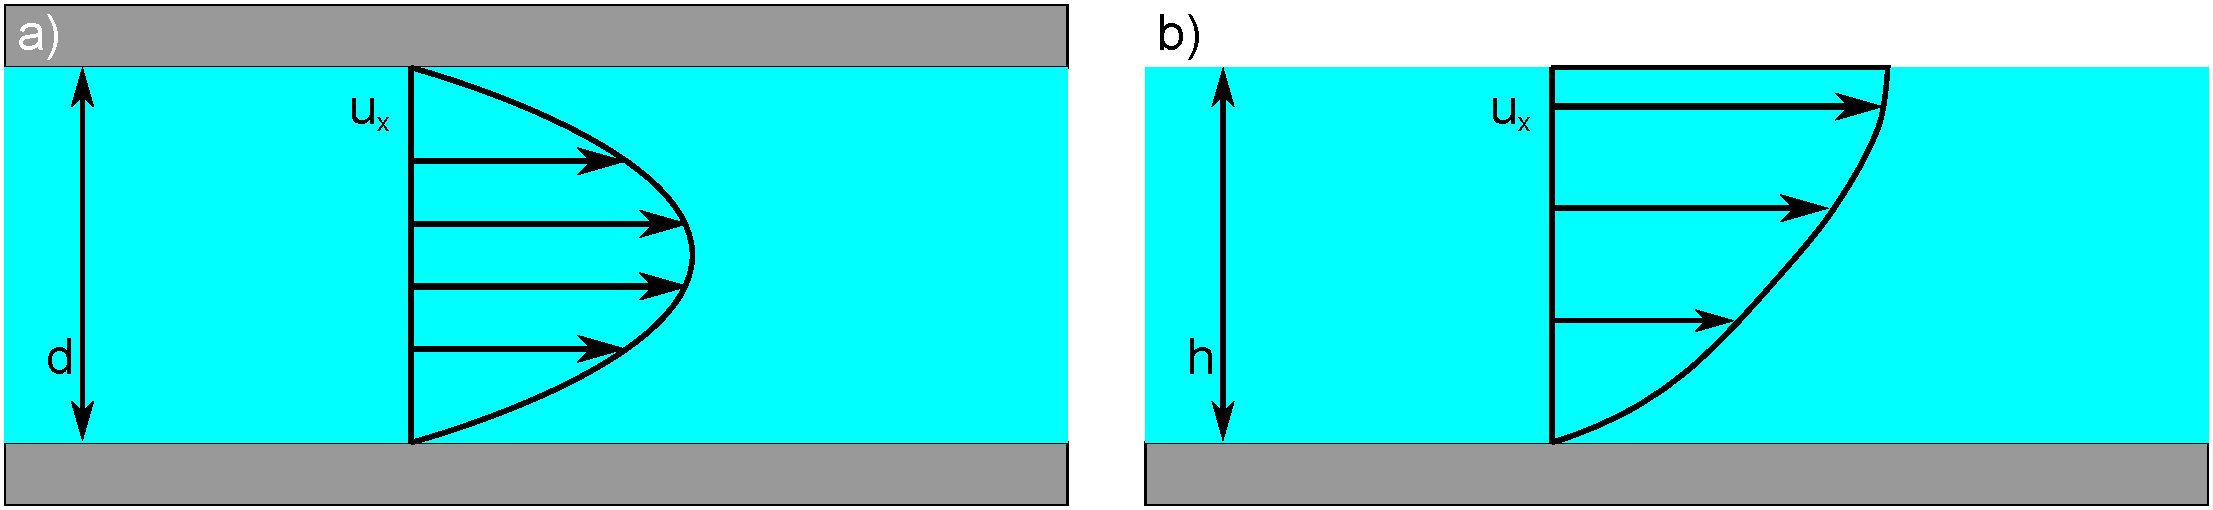
\includegraphics[width=0.95\textwidth]{graphics/Simple_flow.pdf}
    \caption{a) Schematic, cut through the center, velocity profile of a pipe flow with wall friction and no slip boundary condition.
    The flow velocity $u_x$ can be calculated using Eq.~(\ref{eq:pois_vel_profile}).
    b) Similar case in terms of a shallow water geometry. 
    The upper wall is replaced with a pressure free boundary while the lower wall induces friction according to a no-slip boundary condition.
    }
    \label{fig:pois_vel_profile}
\end{figure}
\subsection{Poiseuille flow}
The Poiseuille flow is one amongst those few problems that can be solved analytically~\cite{sutera1993history}.
To have an idea about the flow, one can think about a circular pipe.
The pipe is fully filled with a (Newtonian) liquid, see Fig.~\ref{fig:pois_vel_profile} for an oversimplified illustration.
By an external pressure gradient, for example a pump, a continuous flow is generated.
The velocity profile of this flow can be explained with the equation~\cite{batchelor2000introduction, krueger2017}
\begin{equation}\label{eq:pois_vel_profile}
    u_x(y) = -\frac{\partial_x p}{2\mu}y(y-d),
\end{equation}
where $d$ the diameter of the pipe is.
The profile is parabolic with vanishing $u_x$ at the walls and a maximum at $d/2$. 
Thus the above equation defines the balance between driving force, here the pressure difference, and the friction at the walls.

Coming back to the shallow water picture where no upper wall is present as depicted in Fig.~\ref{fig:pois_vel_profile} b).
The solution is not anymore given by Eq.~(\ref{eq:pois_vel_profile}) but reduces to the half-Poiseuille or Nusselt solution with a new self similar quantity $\bar{h}$~\cite{james2019towards}
\begin{equation}\label{eq:bar_h}
    \bar{h} = \frac{z - b}{h}, \quad \frac{u}{U} = 3\left(\bar{h} - \frac{\bar{h}^2}{2}\right), 
\end{equation}
where $\bar{h}$ is constructed to be in the interval between 0 and 1.
Inserting $\bar{h}$ into Eq.~(\ref{eq:beta_lims}) reveals that the Boussinesq coefficient is given as $\beta = 6/5$, where the integration can be performed using a transformation of the integral measure.
The friction term Eq.~(\ref{eq:sw_bot_friction}) becomes 
\begin{equation}
    \tau_b = \frac{3}{\varepsilon Re}\frac{U}{h} ,
\end{equation}
upon inserting Eqs.~(\ref{eq:bar_h}).
This choice shows a laminar behaviour as the friction term $\tau_b$ depends linearly on $U$ the mean flow velocity.
Interestingly for large Reynolds numbers the friction can become negligible, with the transition to the inviscid shallow water regime.

Two small additions to the friction term $\tau_b$.
When it comes to friction it is often simpler and more accurate to use data from empirical studies or real world experiments.
Within the shallow water literature an often encountered coefficient is the one of Manning, the empirical law that connects flow velocity with friction can be found in ref.~\cite{sturm2021open}.

To close this section we quickly collect the equations that form the shallow water system, see Eqs.~(\ref{eq:shallow_water_cont_true}, \ref{eq:sw_mom_final}).
The generalization of this two dimensional equations towards a second horizontal dimension is straightforward and can be written as~\cite{Salmon:1999:0022-2402:503, PhysRevE.65.036309, thommes2007lattice}
\begin{gather}\label{eq:shallow_water}
        \partial_t h + \nabla \cdot (h\mathbf{u}) = 0, \\
        \partial_t (h\mathbf{u}) + \nabla\cdot (p \mathbb{1} + h\mathbf{u}\mathbf{u} - S) = 0, 
\end{gather}
where the only unknown $\mathcal{S}$ is a yet undefined source term. 
The system Eqs.~(\ref{eq:shallow_water}) concludes the shallow water model. 
In Chap.~\ref{chapter:first_paper} we show how this translates into a numerical solver.

Following in this chapter are two more sections.
The next section and the main point of interest of this work is a short and phenomenological oriented derivation of the thin film model.
In the last section the chapter concludes with a comparison of shallow water with thin film theory.

\section{Lubrication Theory and Thin Films}
\label{sec:thin_films}
Thin liquid films are an interesting problem to study.
Their dynamics is seemingly easy to explain but bare a lot of complexity.
Seemingly easy because everyone has an understanding of soap bubbles and their rather complex bursting mechanics or has seen a rain drop on a plant leaf as motivated in the introduction, Chap.~\ref{chapter:intro}.
Complexity is generated due to the shape of the equation that describes the thin film dynamics, usually a non linear forth order partial differential equation of the film thickness.
When the thickness of a film becomes small, e.g. only a few tens of nanometers the complexity can even be enhanced. 
Complex behaviour can arise due to thermal fluctuations or strictly speaking the mathematical unsolvable problem of moving contact lines e.g. when a wet to dry transition happens.
Similar to the above section's scaling argument and the long wave theory, the Navier-Stokes equation can be reduced to the thin film equation. 
Although with the difference to the shallow water system, see Eqs.~(\ref{eq:shallow_water}), that the thin film equation does only admit a continuity like equation and no accompanying momentum equation~\cite{RevModPhys.69.931, RevModPhys.57.827, RevModPhys.81.1131}.

\begin{figure}
    \centering
    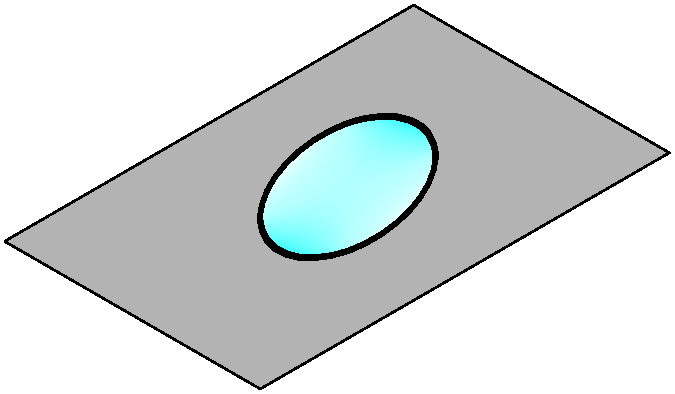
\includegraphics[width=0.95\textwidth]{graphics/contact_line.pdf}
    \caption{Liquid droplet placed on a smooth substrate.
    The three phase contact line which is the interface between the vapor, the solid and liquid phase is displayed as thick black line.}
    \label{fig:contact_line_drop}
\end{figure}
Similar to the shallow water system, the thin film equation only considers the dynamics of a thin liquid \textit{layer} placed on top of a yet undefined surface or substrate.
The defining equation that describes the dynamics of a thin liquid film can be written as~\cite{THIELE2014399, RevModPhys.69.931, RevModPhys.81.1131, RevModPhys.81.739} 
\begin{equation}\label{eq:simple_thin_film}
    \partial_t h = \vec{\nabla}\cdot\left(M(h)\vec{\nabla} p\right).
\end{equation}
Stating that the height can only change if there is a pressure gradient which acts on the film.
In Eq.~(\ref{eq:simple_thin_film}) two unknowns are introduced.
First being the mobility $M(h)$ which determines the exact velocity boundary condition for $h=0$.
Using the no-slip boundary condition, see Eq.~(\ref{eq:no-slip_sw1}), we have 
\begin{equation}\label{eq:no-slip-mobility}
    M(h) = \frac{h^3}{3\mu},
\end{equation}
with $\mu$ being the (dynamic) viscosity, therefore the mobility is inversely proportional to the viscosity.
Of course the velocity boundary condition can be relaxed which is often desired e.g. for contact line movement.
For problems such as dewetting\footnote{Dewetting usually refers to an unstable film which by so-called film rupture recedes into separated droplets. Depending on the film's properties there different modes of dewetting can be identified, such as spinodal or hole nucleation.} it is actually a known approximation to relax the velocity boundary condition at the liquid solid interface~\cite{M_nch_2005, munch2005lubrication, PhysRevLett.95.127801}.
The term contact line or to be precise three-phase contact line defines the single one dimensional interface that connects all three phases involved in the problem, as displayed in Fig.~\ref{fig:contact_line_drop}.
The addition of the parameter $\delta$ makes it possible to interpolate the height of vanishing fluid velocity into the substrate.
Using this interpolation the mobility function Eq.~(\ref{eq:no-slip-mobility}) can be extended towards a slip like behaviour in the proximity of $h\approx 0$ as
\begin{equation}\label{eq:slip_mobility}
    M(h) = \mu^{-1}\left(\frac{h^3}{3} + \delta h^2\right).
\end{equation}

Knowing what the mobility is leaves the pressure term to be the only unknown.
So far the terms surface tension ($\gamma$) or equilibrium contact angle ($\theta_{\text{eq}}$) did not appear.
Because in the first section we did not concern ourselves with a multiphase, multicomponent approach and therefore there was no interface.
In the derivation of the shallow water equations, we encountered an interface, but the hydrostatic pressure defined the interface.
Both theories therefore are not well-equipped to account for either surface tension or balances between surface energies and as such contact angles.
The thin film pressure introduces both of them and can be modelled with
\begin{equation}\label{eq:thin_film_pressure}
    p = -\gamma \Delta h - \Pi(h),
\end{equation}
where $\Delta h$ denotes the two-dimensional Laplacian of the thickness and $\Pi(h)$ is the disjoining pressure functional.
The first term ensures that the fluid's enclosing surface area, the interface between the fluid and vapor phase, is minimal.
The surface tension is therefore the strength with which the surface area minimization is enforced.
$\Pi(h)$, or the disjoining pressure on the other hand takes into account the inter-molecular interactions that can arise, e.g. the interaction between solid substrate and film~\cite{RevModPhys.81.1131, moulton_lega_2013}.
Independent of the exact model the disjoining pressure can be understood as a derivative of an interaction potential.
The model used for this work was first derived by Schwartz and Eley~\cite{SCHWARTZ1998173} and consists of two contributions
\begin{equation}\label{eq:disj_pressure_one}
    \Pi(h) = \kappa f(h),
\end{equation}
where $\kappa$ is a function of material parameters, e.g. surface tension and the contact angle, 
\begin{equation}\label{eq:disj_kappa}
    \kappa = \gamma (1 - \cos\theta) \frac{(n-1)(m-1)}{(n-m)},
\end{equation}
and can be motivated from inter-molecular interactions, see for a rather short description~\cite{MAHADY2015243}.
The second term $f(h)$ is a function of the film thickness.
Here we use a power law with a characteristic height $h_{\ast}$ for which $\Pi(h_{\ast}) = 0$,
\begin{equation}\label{eq:disj_fofh}
    f(h) = \frac{1}{h_{\ast}}\left[\left(\frac{h_{\ast}}{h}\right)^n - \left(\frac{h_{\ast}}{h}\right)^m \right],
\end{equation}
with the constraints that $n>m$ as well as $m > 0$.
This is an effective model for wetting of partially wettable substrates, see Fig.~\ref{fig:wetting_angle}, with a spreading coefficient $S = \gamma_{gs} - \gamma_{ls} - \gamma$ and can be computed as~\cite{Peschka9275}
\begin{equation}\label{eq:disj_spreading}
    S = \int\Pi(h)|_{h=h_{\ast}} \diff h, 
\end{equation}
where different $\gamma$'s denote the different surface energies, e.g. $\gamma_{gs}$ is the surface energy between the gas and the solid phases.
By the very construction of $\Pi(h)$ everything cancels but the factor that contains the contact angle  
\begin{equation}\label{eq:disj_young}
    S = -\gamma(1 - \cos\theta_{\text{eq}}),
\end{equation}\label{eq:Youngs_law}
where we have used Young's law~\cite{doi:10.1098/rstl.1805.0005}
\begin{equation}
    \gamma\cos\theta_{\text{eq}} = \gamma_{gs} - \gamma_{ls},
\end{equation}
as an approximation to the surface energies at equilibrium.
For a perfect wettable substrate the contact angle vanishes and thus $S=0$.
A short side note about interfacial energies, while these can be derived from theory it is almost never possible to measure them accurately in experiments.
What can be measured in experiments on the other hand are the spreading parameter $S$ and/or the Hamaker constant~\cite{RevModPhys.81.739, PhysRevE.93.013120, Peschka9275} 
\begin{figure}
    \centering
    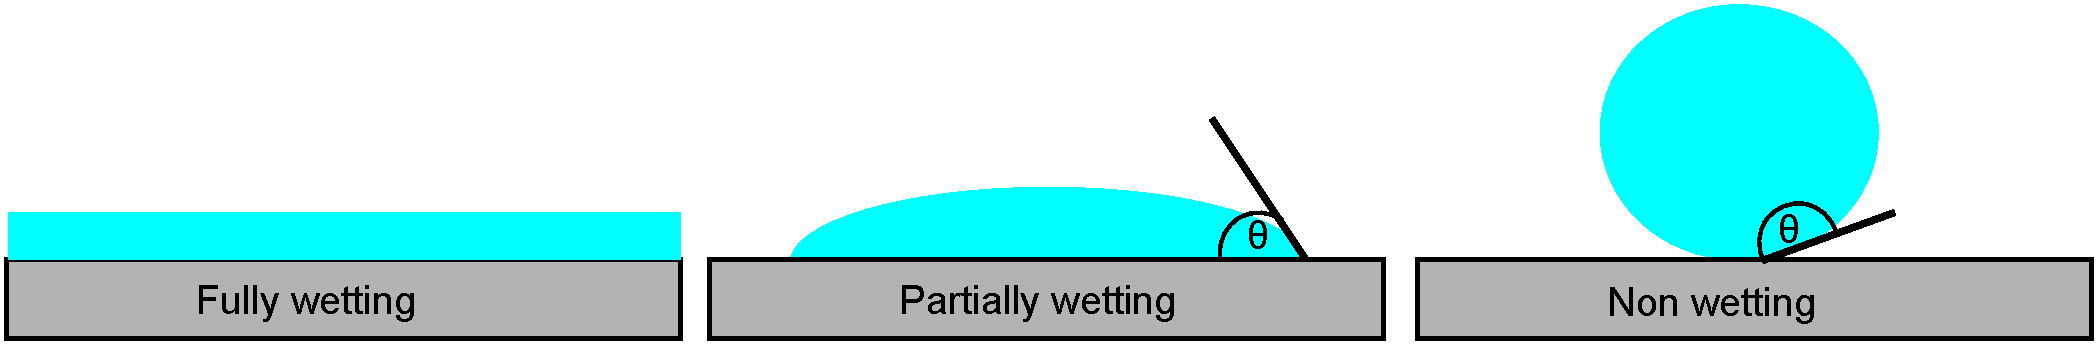
\includegraphics[width=0.95\textwidth]{graphics/Wettings.pdf}
    \caption{Wetting behaviour for different fluid substrate interactions.
    If the affinity between fluid and substrate is very large the substrate is said to be fully wetting with a vanishing contact angle.
    Reducing this affinity, which is usually the case for real substrates, leads to a measurable contact angle and is called partially wetting.
    Surface treatment or complex surface structure can lead to non wetting surfaces, therefore with contact angles of close to $\pi$.}
    \label{fig:wetting_angle}
\end{figure} 

After the introduction of the thin film equation and some phenomenology on it, as such emergence of surface tension and disjoining pressure a more detailed derivation of Eq.~(\ref{eq:simple_thin_film}) is about to follow.
Again the starting point will be the Navier-Stokes equation and the path is not very different from the shallow water derivation.
However there are some differences.

\subsection{Scaling and boundary conditions}
\label{subsec:thin_film_scaling}

Thin liquid films similar to shallow water theory have a spatial dimension which is much smaller than the other two therefore Eq.~(\ref{eq:thickness_length}) is again applicable.
Some instructive everyday example that enforces this understanding would be the thickness of an oil film in a frying pan. 
The pan is about 30cm in diameter while the thickness of the oil film is not even 3cm.
Assuming that the oil is covering the whole surface of the pan $\varepsilon = 1/10 \approx 10^{-1}$.
While very illustrative this example displays interesting physics.
When the pan is heated the film usually ruptures in the middle and a ring-like structure is left as shown in ref.~\cite{doi:10.1063/5.0035547}.

The basic assumption is, again, the absence of strong slopes and therefore
\begin{equation}\label{eq:small_slopes}
    |\vec{\nabla} h| \ll 1,  
\end{equation}
meaning the thickness changes gradually along the two vertical dimensions.
Furthermore the Reynolds numbers for thin film flows are small ($Re < 1$), thus the inertial effects are at most subdominant.

Starting point of the derivation Eq.~(\ref{eq:simple_thin_film}) is the Navier-Stokes, see Eq.~(\ref{eq:navier_stokes_fin}) with the continuity equation~(\ref{eq:incomp}).
Rescaling the quantities according to 
\begin{align}\label{eq:thin_film_scaling}
    \tilde{x} &= \frac{x}{L},\quad \tilde{y} = \frac{y}{L},\quad \tilde{z} = \frac{z}{H},\nonumber \\
    \tilde{u}_x &= \frac{u_x}{U},\quad \tilde{u}_y = \frac{u_y}{U},\quad \tilde{u}_z = \frac{u_z}{V},\nonumber \\
    \tilde{t} &= \frac{L}{U} t,\quad \tilde{p} = \frac{H^2 p}{\mu U L}, 
\end{align}
where $U$ and $V$ are characteristic velocities in the vertical and horizontal direction respectively. 
The scaling factor in front of the pressure can be computed assuming stationary unidirectional flow with $\mathbf{u} = (u(z), 0, 0)$.
In contrast to the shallow water section Sec.~\ref{sec:theory_shallow_water} here all three dimensions are considered.
The motivation for this is the fact that most numerical experiments in Chaps.~\ref{chapter:fourth_paper}-\ref{chapter:third_paper} are done using a two dimensional domain. 
 
Inserting the rescaled quantities the continuity equation becomes
\begin{equation}\label{eq:cont_thin_film_1}
     \nabla\cdot\mathbf{u} = \partial_{\tilde{x}} \tilde{u}_x + \partial_{\tilde{y}} \tilde{u}_y + \frac{V L}{U H}\partial_{\tilde{z}} \tilde{u}_z = 0,
\end{equation}
which means that $V = U H/L$ to ensure all terms are of the same order in $\varepsilon$.
Upon inserting them into the Navier-Stokes equation we get for the x-component only
\begin{align}
     \rho L \partial_{\tilde{t}}\tilde{u}_x &+ \rho\left[\frac{U^2}{L}\left(\tilde{u}_x\partial_{\tilde{x}}\tilde{u}_x + \tilde{u}_y\partial_{\tilde{y}}\tilde{u}_x\right) + \frac{U V}{H}\tilde{u}_z\partial_{\tilde{z}}\tilde{u}_x\right] = \nonumber \\ &-\frac{\mu U}{H^2} \partial_{\tilde{x}} \tilde{p} + \mu\left[\frac{U}{L^2}(\partial^2_{\tilde{x}}\tilde{u}_x + \partial^2_{\tilde{y}}\tilde{u}_x) + \frac{U}{H^2}\partial^2_{\tilde{z}}\tilde{u}_x\right].
\end{align}
For the $y$ and $z$ component we refer to the review by Oron et al.~\cite{RevModPhys.69.931}.
Although the equation is now non-dimensional it is instructive to multiply both sides with $H^2/\mu U$ and collect the characteristic quantities in dimensional less numbers, here the Reynolds number, see Eq.~(\ref{eq:Re_and_Fr}), with $L = H, v_0 = U$ and $\varepsilon$  
\begin{equation}
    \varepsilon Re \left(\partial_{\tilde{t}}\tilde{u}_x + \tilde{u}_x\partial_{\tilde{x}}\tilde{u}_x + \tilde{u}_y\partial_{\tilde{y}}\tilde{u}_x + \tilde{u}_z\partial_{\tilde{z}}\tilde{u}_x \right) = -\partial_{\tilde{x}}\tilde{p} + \varepsilon^2\left(\partial^2_{\tilde{x}}\tilde{u}_x + \partial^2_{\tilde{y}}\tilde{u}_x\right) + \partial^2_{\tilde{z}}\tilde{u}_x. 
\end{equation}
Both the Reynolds number as well as $\varepsilon$ are by definition small. 
Therefore the terms with higher order in $\varepsilon$ are at most subleading.
Collecting only the term of $O(1)$ and performing the same scaling for the two other directions leads to the non-dimensional momentum equation of a thin film on a solid substrate
\begin{align}
    -\partial_{\tilde{x}}\tilde{p} + \partial^2_{\tilde{z}}\tilde{u}_x &= 0,  \label{eq:thin_film_pressure_x}\\
    -\partial_{\tilde{y}}\tilde{p} + \partial^2_{\tilde{z}}\tilde{u}_y &= 0,  \label{eq:thin_film_pressure_y}\\
    \partial_{\tilde{z}}\tilde{p} &= 0. \label{eq:thin_film_pressure_z}
\end{align}
where for the last of the above equations the analogy to the shallow water model can be drawn using Eq.~(\ref{eq:hydrostat_sw_euler}) which states that the pressure gradient does not depend on $z$.
 
The system so far does not resemble Eq.~(\ref{eq:simple_thin_film}).
Therefore some more derivation is in order, starting with the application of the boundary conditions.
Between the fluid and solid phase a no-slip boundary condition is used, therefore analogue to Eq.~(\ref{eq:no-slip_sw1},\ref{eq:no-slip_sw2}) we have
\begin{equation}\label{eq:thin_all_v_noslip}
    \mathbf{u}|_{z=0} = \mathbf{0},    
\end{equation}
and for the vapor fluid interface a stress balance need to be satisfied~\cite{leal2007advanced}
\begin{equation}\label{eq:thin_film_upper_bc}
    (\tilde{\sigma}_l - \tilde{\sigma}_v)\cdot\mathbf{n} + \nabla_S\gamma - \gamma\mathbf{n}(\nabla\cdot\mathbf{n}) = 0,
\end{equation}
where $\tilde{\sigma}_{l,v}$ are the stress tensors for the liquid ($l$) and vapor ($v$) phase. 
Further we have the normal vector $\mathbf{n}$ along the fluid interface and the surface gradient $\nabla_S$.
The two surface tension terms account for changes along the surface ($\nabla_S$) and the Laplace pressure due the curvature ($\kappa$) of the liquid air interface $2\kappa = \nabla\cdot\mathbf{n}$.
The stress tensor for a Newtonian liquid has been defined in Eq.~(\ref{eq:total_stress}) and for the sake of completeness is given as 
\begin{gather}\label{eq:stress_matrix}
    \tilde{\sigma} = \begin{pmatrix}
    -p + 2\mu\partial_x u_x & \mu(\partial_y u_x + \partial_x u_y) & \mu(\partial_z u_x + \partial_x u_z) \\
    \mu(\partial_x u_y + \partial_y u_x) & -p + 2\mu\partial_y u_y & \mu(\partial_z u_y + \partial_y u_z) \\
    \mu(\partial_x u_z + \partial_z u_x) & \mu(\partial_y u_z + \partial_z u_y) & -p + 2\mu\partial_z u_z   
    \end{pmatrix} ,
\end{gather}
in matrix notation.
The normal vector $\mathbf{n}$ is defined as 
\begin{equation}\label{eq:normal_vec_thin_film}
    \mathbf{n} = \frac{1}{\sqrt{1 + (\partial_x h)^2 + (\partial_y h)^2}}(-\partial_x h, -\partial_y h, 1).
\end{equation}
Computing the inner product of Eq.~(\ref{eq:thin_film_upper_bc}) with the normal vector $\mathbf{n}$ yields
\begin{equation}\label{eq:balance_stresses_normal}
    p_v - p -(\mathbf{n}\cdot\mathbf{T})\cdot\mathbf{n} + \gamma\mathbf{n}(\nabla\cdot\mathbf{n})\cdot\mathbf{n} = 0,
\end{equation}
where $p_v$ is the pressure in the vapor phase and $\mathbf{T} = \mu(\nabla\mathbf{u} + \nabla\mathbf{u}^T)$.
In fact only the contribution from the liquid is considered, because $\mu_l \gg \mu_v$.
Assuming a water air interface we have a ratio of dynamic viscosity $\mu_{air} / \mu_{\ce{H2O}} = 0.018/ 1.0016 \approx 0.02$.
Inserting the scaling defined in the Eq.~(\ref{eq:thin_film_scaling}) and collecting only leading order contributions we have 
\begin{equation}
    \tilde{p} = p_v + P - \gamma(\partial_{\tilde{x}}^2 h + \partial_{\tilde{y}}^2 h),
\end{equation}
where $P$ accounts for all additional contributions to the pressure, e.g. the hydrostatic pressure, see for examples Eq.~(\ref{eq:hydro_static_int}), but as well for the disjoining pressure $\Pi(h)$ Eq.~(\ref{eq:disj_pressure_one}).

Now that the normal stresses are balanced at the fluid vapor interface the same has to be done for the tangential stresses.
Therefore taking Eq.~(\ref{eq:thin_film_upper_bc}) and multiplying it with the tangential unit vectors $\mathbf{t}_i$ 
\begin{equation}\label{eq:upper_bc_tangential}
    \mathbf{t}_i(\mathbf{T}_l - \mathbf{T}_v)\cdot\mathbf{n} + \mathbf{t}_i\cdot\nabla_S\gamma = 0.
\end{equation}
Using the same argument as above, therefore having a high viscosity contrast between the liquid and vapor phase contributions associated with $\mathbf{T}_v$ are neglected.
Collecting leading order terms one gets
\begin{align}
    \mu\partial_{\tilde{z}}\tilde{u}_x = \tau_x, \label{eq:tau_x_thin}\\
    \mu\partial_{\tilde{z}}\tilde{u}_y = \tau_y, \label{eq:tau_y_thin}
\end{align}
Having defined the leading order equations for the flow velocity, the next step is integrate them along the vertical dimension.

\subsection{Vertical integration}
\label{subsec:thin_film_int}
The system of equations so far do not resemble Eq.~(\ref{eq:simple_thin_film}).
A crucial step is missing, actually the same step that happen in Sec.~\ref{subsec:int_sw}, namely the integration along the vertical.
\begin{align}\label{eq:int_vels_thin}
    \int_0^h\int_0^h (-\partial_x p + \partial_z^2 u_x ) \diff^2 z = 0,  \\
    \int_0^h\int_0^h (-\partial_y p + \partial_z^2 u_y ) \diff^2 z = 0. 
\end{align}
This however can readily be done as we know that the pressure does not depend on $z$, see Eq.~(\ref{eq:thin_film_pressure_z}). 
Therefore Eqs.~(\ref{eq:thin_film_pressure_x}, \ref{eq:thin_film_pressure_y}) integrated twice with respect to $z$ yields
\begin{align}
    u_x = \frac{\partial_x p}{2\mu}(z^2 - 2hz) + \frac{\tau_x z}{\mu}, \label{eq:vel_x_int_thin}\\
    u_y = \frac{\partial_y p}{2\mu}(z^2 - 2hz) + \frac{\tau_y z}{\mu}, \label{eq:vel_y_int_thin}
\end{align}
where the integration constants were determined using the boundary conditions Eqs.~(\ref{eq:thin_all_v_noslip}, \ref{eq:tau_x_thin}, \ref{eq:tau_y_thin}) and due to convenience the tilde has been dropped.
In the following many steps are fairly similar to the derivation of Sec.~\ref{sec:theory_shallow_water} however never the less it is instructive to proceed step by step.
Performing another integration of the velocities with respect to the thickness to compute the discharge $Q$ or volume flux 
\begin{align}
    Q_x = \int_0^h u_x(z)\diff z = -\frac{h^3}{3\mu}\partial_x p + \frac{h^2}{2\mu} \tau_x, \label{eq:discharge_thin_x} \\
    Q_y = \int_0^h u_y(z)\diff z = -\frac{h^3}{3\mu}\partial_y p + \frac{h^2}{2\mu} \tau_y, \label{eq:discharge_thin_y}
\end{align}
where due to the no slip boundary condition the mobility function $M(h)$, Eq.~(\ref{eq:no-slip-mobility}) naturally arises.

Now that the horizontal velocities are know we use them to solve the integration of the continuity equation Eq.~(\ref{eq:incomp})
\begin{equation}\label{eq:cont_thin}
    \int_0^h(\partial_x u_x + \partial_y u_y + \partial_z u_z) = 0,
\end{equation}
making use of the Leibniz rule one more time and showing only the $u_x$ component
\begin{equation}
    \int_0^h \partial_x u_x(z) \diff z = \partial_x\int_0^h u_x\diff z + 0 - \partial_x h u_x(h) = \partial_x Q_x - \partial_x h u_x(h),  
\end{equation}
where Eq.~(\ref{eq:discharge_thin_x}) was used.
Inserting the above equation for the $x$ and $y$-component into the Eq.~(\ref{eq:cont_thin}) and performing the integration of $\partial_z u_z$ yields
\begin{equation}\label{eq:thin_dummy}
    \partial_x Q_x - (\partial_x h) u_x(h) + \partial_y Q_y - (\partial_y h) u_y(h) + u_z(h) - u_z(0) = 0.
\end{equation}
Using the no-slip boundary condition does allow to get rid of $u_z(0) = 0$.
The upper bound $u_z(h)$ can be computed using the material derivative, see Eq.~(\ref{eq:mat_dev}). 
Using a similar approach to the height as in Eq.~(\ref{eq:shallow_water_height}) with $f(\vec{x},t) = h(\vec{x},t) - z$, which is $0$ at  the interface yields
\begin{equation}\label{eq:mat_uz_h}
    D_t f = \partial_t h + u_x\partial_x h + u_y\partial_y h - u_z = 0.
\end{equation}
Inserting the found result for $u(h)$ into Eq.~(\ref{eq:thin_dummy}) we get
\begin{equation}\label{eq:thin_obsc}
    \partial_x Q_x + \partial_y Q_y + \partial_t h = 0,
\end{equation}
which is almost the same as Eq.~(\ref{eq:simple_thin_film}).
Inserting the $Q$'s, therefore Eqs.~(\ref{eq:discharge_thin_x},\ref{eq:discharge_thin_y}) yields
\begin{equation}
    \partial_t h = \vec{\nabla}\cdot\left(\frac{h^3}{3\mu}\vec{\nabla} p + \frac{h^2}{2\mu}\tau\right),
\end{equation}
which compared to Eq.~(\ref{eq:simple_thin_film}) includes the shear contribution $\tau$.
Assuming the interface is not accelerated (e.g. in case of dewetting) the shear term can be neglected and the resulting equation is 
\begin{equation}\label{eq:thin_final}
    \partial_t h(\vec{x},t) = \vec{\nabla}\cdot\left(\frac{h^3}{3\mu}\vec{\nabla} p\right).
\end{equation}

With this derivation of both models, be it the shallow water system or the thin film equation, from the Navier-Stokes equation is complete.
Of course this derivation comes short if there is addition dynamics such as thermal fluctuations, see Chap.~\ref{chapter:second_paper} for a analysis of their impact on dewetting.

Because the thin film equation is the main point of entry for the following chapters it is instructive to derive some more phenomenology of Eq.~(\ref{eq:thin_final}).
Therefore in the next section a short derivation of linear stability of Eq.~(\ref{eq:thin_final}) is performed.

\subsection{Linear stability analysis}
\label{susbsec:Lin_stab}
The concept of the linear stability analysis is a rather interesting one.
One asks the questions what happens to the system, e.g. the thin film equation, if a small perturbation is added to some stable solution.
Will the system come back to the stable solution and therefore damp out the perturbation or will the system become unstable and open up a new branch in the phase space of solutions?

A simple example for this can be the string of a guitar.
In the rest case, which forms a stable solution for the length of the string, the string is flat.
If one gently touches the string a small perturbation is added and will undulate the string such that it starts to vibrate.
The vibrations will turn in to waves with well defined wavelengths. 
Most of them will be damped and only one wavelength or better wavemode will survive.
The sound related to that wavemode defines the eigenmode of the string.
Due to friction and boundary conditions the string will come go back to be flat.
Which means that the string is linearly stable.

Using this analysis for the thin film equation we simply add a small perturbation to a flat film with
\begin{equation}\label{eq:lin_stab_delta}
    h(\vec{x},t) = h_0 + \delta h(\vec{x},t),
\end{equation}
where $h_0$ is the thickness of the flat film and $\delta h$ is the small, but dynamic perturbation.
Small in this sense means that $\delta h \ll h_0$.
Now we follow the development of the perturbation and therefore quantify the stability of the system.
The term linear in linear stability analysis comes from the fact that one considers only terms up to $O(\delta h)$, but neglects higher orders of $\delta h$~\cite{laugesen2000linear}.

Inserting Eq.~(\ref{eq:lin_stab_delta}) into Eq.~(\ref{eq:thin_final}) yields
\begin{equation}\label{eq:stab_1}
    \partial_t (h_0 + \delta h) = \vec{\nabla}\cdot\left\{\frac{(h_0 + \delta h)^3}{3\mu}\vec{\nabla} [-\gamma\vec{\Delta}(h_0 + \delta h) - \Pi(h_0 + \delta h)]\right\},
\end{equation}
where the pressure term has been written explicitly in terms of Laplace and disjoining pressure.
Using the fact that $h_0$ is constant and thus $\vec{\nabla} h_0 = \partial_t h_0= 0$ we can compute the derivatives
\begin{equation}\label{eq:stab_2}
    \partial_t \delta h = \frac{h_0^3}{3\mu}\left[-\Pi'(h_0)\vec{\nabla}^2\delta h -\gamma\vec{\nabla}^4\delta h\right],
\end{equation}
where $\Pi'(h_0)$ is a short notation for
\begin{equation}\label{eq:deriva_Pi}
    \Pi'(h_0) = \frac{\partial\Pi(h)}{\partial h}\bigg\rvert_{h=h_0}.
\end{equation}

Instead of solving this equation in real space it is simpler and more instructive to solve it in Fourier space.
Which means that a wavelength $\lambda$ in real space becomes a wavemode $q$ in Fourier space. 
Fourier transforming the perturbation $\delta h$ we have 
\begin{equation}\label{eq:fourier_h}
    \tilde{\delta h}(\vec{q},t) = \int_{-\infty}^{\infty} \delta h(\vec{x},t) e^{-i\vec{x}\cdot\vec{q}} \diff\vec{x}.    
\end{equation}
Further performing the Fourier transformation on Eq.~(\ref{eq:stab_2}), mainly interchanging $\vec{\nabla} \rightarrow \vec{q}$ yields
\begin{equation}\label{eq:stab_3}
    \partial_t \tilde{\delta h}(\vec{q},t) = \frac{h_0^3}{3\mu}\left[-\Pi'(h_0)\vec{q}^2\delta h -\gamma\vec{q}^4\delta h\right].
\end{equation}
From the above equation one can readily read the dispersion relation $\omega(q)$ by 
\begin{align}
    \partial_t \tilde{\delta h} &= \omega(q)\tilde{\delta h}, \\
    \omega(q) &= \frac{h_0^3}{3\mu}\left[-\Pi'(h_0)q^2 -\gamma q^4\right], 
\end{align}
where $q = \sqrt{q_x^2 + q_y^2}$.
To find the maximal unstable wavemode $q_0$ or put simply the eigenmode of the (spinodally dewetting) film we set the left hand side equal with $0$ and solve for $q$
\begin{align}\label{eq:stab_4}
    \partial_t \tilde{\delta h} &= 0, \\
    \frac{h_0^3}{3\mu}q^2\left[-\Pi'(h_0)\delta h -\gamma q^2\delta h\right] &= 0, \\
    -\Pi'(h_0) -\gamma q^2 &= 0, \\
    q_0 &= \sqrt{\frac{-\Pi'(h_0)}{\gamma}} .
\end{align}

An example of a dispersion relation which follows the above equation is shown in Fig.~\ref{fig:dispertion_1}.
Wavemodes larger than $q_0$ are damped out as predicted while wavemodes smaller than $\sqrt{2q_0}$ are growing with a maximum at $q_0$.
A characteristic time scale of the problem is given as
\begin{equation}
    t_0 = \frac{3\mu}{\gamma h_0^3 q_0^4},
\end{equation}
with is used to normalize the time in Fig.~\ref{fig:dispertion_1}.
Because the concept of linear stability is such an important one, we encounter it again in Chap.~\ref{chapter:first_paper} see Fig.~\ref{fig:RTI} as well as in Chap.~\ref{chapter:second_paper} see Figs.~\ref{fig:theory_simulation_structure_factor}, \ref{fig:spectral_analysis_deter_sine8}, \ref{fig:spectral_analysis_stoch_sine8}, \ref{fig:square_wave_both}.
Chapter~\ref{chapter:second_paper} deals solemnly with the addition of a fluctuating term and the so called stochastic thin film equation.
The new term due to thermal fluctuations offers some interesting features on both the structure factor as well as the dispersion.

\begin{figure}
    \centering
    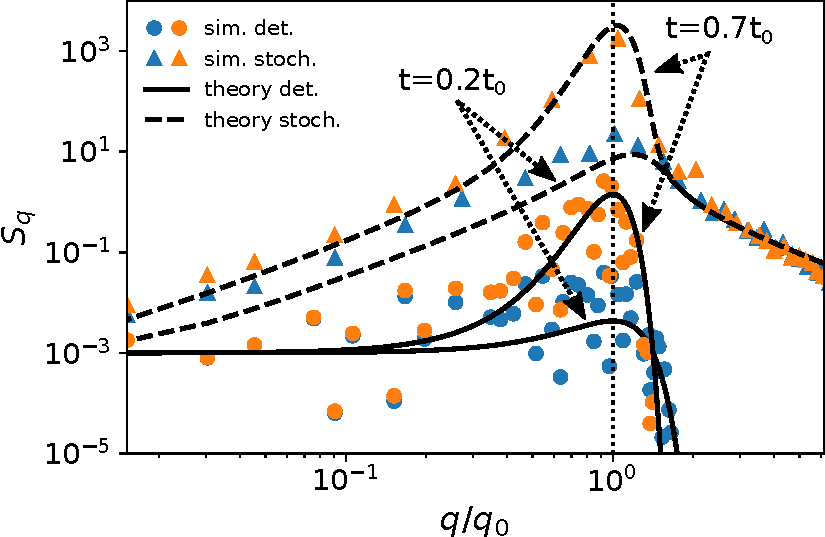
\includegraphics[width=0.95\textwidth]{graphics/spectratheta20.pdf}
    \caption{Dispersion relation of a spinodally dewetting thin film with and without thermal fluctuations.
    Where $S(q)$ is the structure factor depending on the wavemode $q$.
    The dots and triangles are generated using the here presented numerical method. 
    Full and dashed line are the theoretical prediction based on Eq.~(\ref{eq:simple_thin_film}) and its fluctuating extension, Eq.~(\ref{eq:structure_factor_2}).
    }
    \label{fig:dispertion_1}
\end{figure}
% \subsection{The stochastic thin film equation}
% \label{subsec:stoch_thin_film}
% In Chap.~\ref{chapter:second_paper} the stochastic thin film equation is the main point of interest. 
% We study the effects the that thermal fluctuations induces on a dewetting of thin film.
% These fluctuations are usually neglected because their amplitude is small.
% Taking a look at the free mean path of a particle we have
% \begin{equation}\label{eq:thermal_wavelenght}
%     \lambda_{k_BT} = \frac{\mu}{\rho}\sqrt{\frac{\pi k_BT}{2m}},
% \end{equation}
% where $m$ is the mass of the particle.
% Crunching number yields a free mean path $\lambda_{k_BT} \approx 100$nm and thus usually much smaller than any 

% The stochastic or fluctuating thin film equation (STF) is generalization of the thin film equation with the addition of thermal fluctuations.

\section{Differences and Overlap}
\label{sec:shallow_to_thin}

In the last section of this chapter a quick recap of the two theories, name the shallow water model and the thin film equation. 
Theoretical starting point of this chapter is the Navier-Stokes equation, as such the equation of motion for a fluid.
This equation does not allow for a general solution, as of today.
One way out of this mess is to \textit{brute} force an approximation with numerical methods as will be discussed in the next chapter~\ref{chapter:method}.
On the other hand, what I would call the Physics approach is to make approximations directly at the equation.

In Sec.~\ref{sec:theory_shallow_water} the main idea behind behind the shallow water system is that one needs to care only about a thin column of fluid.
With the crucial introduction of the scaling parameter $\varepsilon$, see Eq.~(\ref{eq:thickness_length}), it is possible to derive a different first continuity equation and momentum equation, see Eqs.~(\ref{eq:shallow_water}).
However instead of the fluids density $\rho(\mathbf{x},t)$ one is left with a height $h(\vec{x},t)$ due to the vertical integration.
Apart from that the shallow water covers all nearly all ranges of geophysical flows, from slowly creeping lava to quickly evolving weather systems.
The theory is not limited to vanishing or small $Re$ and captures phenomena such as Tsunami waves (therefore soliton like solutions). 
Within this model, the fluids viscosity is at most subleading.
Which does not mean that there are no models considering the fluids viscosity.
The main source of friction is the interaction with the ground.
Surface tension as well is usually not considered, which is arguably irrelevant for weather systems.

The thin film equation Sec.~\ref{sec:thin_films} is build upon a similar argument.
It's derivation and first development however did serve another purpose as mentioned in the introduction.
Nevertheless the thin film equation, requires similar to the shallow water model a single spatial dimension which is much smaller than the others.
While the shallow water does allow for broader range of applications the thin film equation does serve a single purpose.
And that single purpose is the regime of flows in the low $Re$ and $Ca$ regime, not to confuse with Stokes regime.
Creeping flows or wetting and dewetting phenomena are the use cases of the thin film equation.
Dominant contributions are Laplacian pressure which is enforced by the surface tension.
As the flows are slow and liquids have negligible inertia the viscosity is an important factor.

In Chap.~\ref{chapter:first_paper} we ask the question if these two theories can be merged.
The clear answer to this question is, yes they can.
What is important however is the exact knowledge of flow regime, because to match these two one needs to make crude assumptions.
If this assumptions are violated there is no guaranty that a result is correct.